
% ----------------------------------------------------------------------
%                   LATEX TEMPLATE FOR PhD THESIS
% ----------------------------------------------------------------------

% based on Harish Bhanderi's PhD/MPhil template, then Uni Cambridge
% http://www-h.eng.cam.ac.uk/help/tpl/textprocessing/ThesisStyle/
% corrected and extended in 2007 by Jakob Suckale, then MPI-CBG PhD programme
% and made available through OpenWetWare.org - the free biology wiki


%: Style file for Latex
% Most style definitions are in the external file PhDthesisPSnPDF.
% In this template package, it can be found in ./Latex/Classes/
\documentclass[twoside,11pt]{Latex/Classes/PhDthesisPSnPDF}


%: Macro file for Latex
% Macros help you summarise frequently repeated Latex commands.
% Here, they are placed in an external file /Latex/Macros/MacroFile1.tex
% An macro that you may use frequently is the figuremacro (see introduction.tex)
\include{Latex/Macros/MacroFile1}



%: ----------------------------------------------------------------------
%:                  TITLE PAGE: name, degree,..
% ----------------------------------------------------------------------
% below is to generate the title page with crest and author name

%if output to PDF then put the following in PDF header
%DONT FORGET TO PUT THIS DATA
\ifpdf  
    \pdfinfo { /Title  (Title of your Thesis)
               /Creator (TeX)
               /Producer (pdfTeX)
               /Author (YourName your@email.net)
               /CreationDate (D:YYYYMMDDhhmmss)  %format D:YYYYMMDDhhmmss
               /ModDate (D:YYYYMMDDhhmm)
               /Subject (xyz)
               /Keywords (add, your, keywords, here) }
    \pdfcatalog { /PageMode (/UseOutlines)
                  /OpenAction (fitbh)  }
\fi


\title{UNIVERSITY OF TARTU \\
	FACULTY OF MATHEMATICS AND COMPUTER SCIENCE \\
	Institute of Computer Science}



% ----------------------------------------------------------------------
% The section below defines www links/email for author and institutions
% They will appear on the title page of the PDF and can be clicked
\ifpdf
  \author{\href{mailto:email@ut.ee}{Your Name}}
%  \cityofbirth{born in XYZ} % uncomment this if your university requires this
%  % If city of birth is required, also uncomment 2 sections in PhDthesisPSnPDF
%  % Just search for the "city" and you'll find them.
  \collegeordept{\href{http://www.something.net}{CollegeOrDepartment}}
  \university{\href{http://www.something.net}{University}}

  % The crest is a graphics file of the logo of your research institution.
  % Place it in ./0_frontmatter/figures and specify the width
  \crest{\includegraphics[width=4cm]{logo}}
  
% If you are not creating a PDF then use the following. The default is PDF.
\else
  \author{YourName}
%  \cityofbirth{born in XYZ}
  \collegeordept{CollegeOrDept}
  \university{University}
  \crest{\includegraphics[width=4cm]{logo}}
\fi

%\renewcommand{\submittedtext}{change the default text here if needed}
\degree{Philosophi\ae Doctor (PhD), DPhil,..}
\degreedate{year month}


% ----------------------------------------------------------------------
       
% turn of those nasty overfull and underfull hboxes
\hbadness=10000
\hfuzz=50pt

%: --------------------------------------------------------------
%:                  NEW COMMANDS: definitions
% --------------------------------------------------------------

\newcommand{\HRule}{\rule{\linewidth}{0.5mm}}

%: --------------------------------------------------------------
%:                  FRONT MATTER: dedications, abstract,..
% --------------------------------------------------------------

\begin{document}




%\language{english}

% sets line spacing
\renewcommand\baselinestretch{1.2}
\baselineskip=18pt plus1pt


%: ----------------------- generate cover page ------------------------

%\maketitle  % command to print the title page with above variables


%: ----------------------- cover page back side ------------------------
% Your research institution may require reviewer names, etc.
% This cover back side is required by Dresden Med Fac; uncomment if needed.

%\newpage
%\vspace{10mm}
%1. Reviewer: Name

%\vspace{10mm}
%2. Reviewer: 

%\vspace{20mm}
%Day of the defense:

%\vspace{20mm}
%\hspace{70mm}Signature from head of PhD committee:


%: ----------------------- Here comes the UT first page ------------------------

\begin{titlepage}

\begin{center}

\large
UNIVERSITY OF TARTU\\[2mm]
 
\uppercase{Faculty of Mathematics and Computer Science}\\[2mm]
Institute of Computer Science\\
Computer Science\\[2mm]

\vspace{25mm}


% Title
%\HRule \\[0.4cm]
\Large Enno Eller

\vspace{4mm}

\huge Simplifying Mobile Social Media Authentication On Android

\vspace{20mm}

\Large Bachelor Thesis (6 ECTS)

\end{center}

\vspace{2mm}

\begin{flushright}
 {
 \setlength{\extrarowheight}{5pt}
 \begin{tabular}{r l} 
  \sffamily Supervisor: & \sffamily Huber Flores, MSc \\
  \sffamily Supervisor: & \sffamily Satish Srirama, PhD
 \end{tabular}
 }
\end{flushright}

\vfill

\centerline{Tartu, 2015}

\end{titlepage}


%: ----------------------- abstract ------------------------

% Your institution may have specific regulations if you need an abstract and where it is to be placed in the document. The default here is just after title.

\noindent\textbf{\large Simplifying Mobile Social Media Authentication On Android}
\vspace*{2ex}
{\flushleft{\textbf{Abstract:}}}

\noindent Nowadays, smartphones are very common and people all around the world are using them in their everyday life. Even though mobile phones were originally invented as calling devices, smartphones allow the user to communicate in different ways including social media, instant messaging, recording and watching videos, etc. Recent statistics as of January 2014 claim, that 74\% of online adults use social media. In case they own a smartphone, they probably use social media on it as well, but with restrictions that come with the size of the device, affecting how we view content and also type. Typing on smartphones can be frustrating, but more so when the keyboard size prevents us from succeeding with authentication and we have to type the same text numerous times, which can lead to shorter passwords decreasing the security of the accounts. This paper proposes a solution to such occurrences by using pattern recognition rather than typing. Patterns allow the screen to be used more efficiently, giving the user more room for accuracy errors. Survey results indicate that approaching authentication in this way is feasible.

\vspace*{2ex}

{\flushleft{\textbf{Keywords:} Mobile, Android, Authentication, Pattern}}

\vspace*{3ex}

\noindent\textbf{\large Mobiilse Sotsiaalmeedia Autentimise Lihtsustamine Androidil}
\vspace*{2ex}
{\flushleft{\textbf{L\"{u}hikokkuv\~{o}te:}}}

\noindent T\"{a}nap\"{a}eval on nutitelefonid v\"{a}ga levinud ja k\~{o}ikjal maailmas inimesed kasutavad neid oma igap\"{a}eva elus. Kuigi mobiiltelefonid loodi algselt helistamiseks, nutitelefonid v\~{o}imaldavad kasutajal suhelda erinevatel viisidel, nende seas sotsiaalmeedia, kiirs\~{o}numid, lindistada ja vaadata videoid jne. Hiljutised uuringud jaanuarist 2014 v\"{a}idavad, et 74\% internetti kasutavatest t\"{a}isealistest tarvitavad ka sotsiaalset meediat. Juhul, kui need isikud omavad nutitelefoni, on t\~{o}en\"{a}osus, et nad kasutavad sotsiaalmeediaid ka oma nutiseadmel, kuid piirangutega, mis tulenevad seadme suurusest. Suurus m\~{o}jutab, kuidas me infot vaatame ja teksti sisestame. Tr\"{u}kkimine nutitelefonil v\~{o}ib osutuda masendavaks, seda enam, kui klaviatuuri suurus takistab meil autentimise edu ja me peame sama teksti sisestama mitmeid kordi. Sellised olukorrad v\~{o}ivad viia l\"{u}hemate paroolide kasutamiseni, mis omakorda v\"{a}hendab meie kontode turvalisust. Antud t\"{o}\"{o} pakub v\"{a}lja lahenduse sellistele olukordadele kasutades tr\"{u}kkimise asemel mustreid. Mustrid v\~{o}imaldavad efektiivsemat ekraani kasutust, mis annavad kasutajale rohkem ruumi t\"{a}psuse vigade v\"{a}ltimiseks. Uuringu tulemused n\"{a}itavad, et selline l\"{a}henemine autentimisele on v\~{o}imalik.

\vspace*{2ex}

{\flushleft{\textbf{V\~{o}tmes\~{o}nad:} Mobiilne, Android, Autentimine, Muster}}

% The original template provides and abstractseparate environment, if your institution requires them to be separate. I think it's easier to print the abstract from the complete thesis by restricting printing to the relevant page.
% \begin{abstractseparate}
%   \noindent\textbf{\large Simplifying Mobile Social Media Authentication On Android}
\vspace*{2ex}
{\flushleft{\textbf{Abstract:}}}

\noindent Nowadays, smartphones are very common and people all around the world are using them in their everyday life. Even though mobile phones were originally invented as calling devices, smartphones allow the user to communicate in different ways including social media, instant messaging, recording and watching videos, etc. Recent statistics as of January 2014 claim, that 74\% of online adults use social media. In case they own a smartphone, they probably use social media on it as well, but with restrictions that come with the size of the device, affecting how we view content and also type. Typing on smartphones can be frustrating, but more so when the keyboard size prevents us from succeeding with authentication and we have to type the same text numerous times, which can lead to shorter passwords decreasing the security of the accounts. This paper proposes a solution to such occurrences by using pattern recognition rather than typing. Patterns allow the screen to be used more efficiently, giving the user more room for accuracy errors. Survey results indicate that approaching authentication in this way is feasible.

\vspace*{2ex}

{\flushleft{\textbf{Keywords:} Mobile, Android, Authentication, Pattern}}

\vspace*{3ex}

\noindent\textbf{\large Mobiilse Sotsiaalmeedia Autentimise Lihtsustamine Androidil}
\vspace*{2ex}
{\flushleft{\textbf{L\"{u}hikokkuv\~{o}te:}}}

\noindent T\"{a}nap\"{a}eval on nutitelefonid v\"{a}ga levinud ja k\~{o}ikjal maailmas inimesed kasutavad neid oma igap\"{a}eva elus. Kuigi mobiiltelefonid loodi algselt helistamiseks, nutitelefonid v\~{o}imaldavad kasutajal suhelda erinevatel viisidel, nende seas sotsiaalmeedia, kiirs\~{o}numid, lindistada ja vaadata videoid jne. Hiljutised uuringud jaanuarist 2014 v\"{a}idavad, et 74\% internetti kasutavatest t\"{a}isealistest tarvitavad ka sotsiaalset meediat. Juhul, kui need isikud omavad nutitelefoni, on t\~{o}en\"{a}osus, et nad kasutavad sotsiaalmeediaid ka oma nutiseadmel, kuid piirangutega, mis tulenevad seadme suurusest. Suurus m\~{o}jutab, kuidas me infot vaatame ja teksti sisestame. Tr\"{u}kkimine nutitelefonil v\~{o}ib osutuda masendavaks, seda enam, kui klaviatuuri suurus takistab meil autentimise edu ja me peame sama teksti sisestama mitmeid kordi. Sellised olukorrad v\~{o}ivad viia l\"{u}hemate paroolide kasutamiseni, mis omakorda v\"{a}hendab meie kontode turvalisust. Antud t\"{o}\"{o} pakub v\"{a}lja lahenduse sellistele olukordadele kasutades tr\"{u}kkimise asemel mustreid. Mustrid v\~{o}imaldavad efektiivsemat ekraani kasutust, mis annavad kasutajale rohkem ruumi t\"{a}psuse vigade v\"{a}ltimiseks. Uuringu tulemused n\"{a}itavad, et selline l\"{a}henemine autentimisele on v\~{o}imalik.

\vspace*{2ex}

{\flushleft{\textbf{V\~{o}tmes\~{o}nad:} Mobiilne, Android, Autentimine, Muster}}
% \end{abstractseparate}


%: ----------------------- tie in front matter ------------------------

%\frontmatter
%\include{0_frontmatter/dedication}
%\include{0_frontmatter/acknowledgement}


%: ----------------------- contents ------------------------

\setcounter{secnumdepth}{3} % organisational level that receives a numbers
\setcounter{tocdepth}{3}    % print table of contents for level 3
\tableofcontents            % print the table of contents
% levels are: 0 - chapter, 1 - section, 2 - subsection, 3 - subsection


%: ----------------------- list of figures/tables ------------------------

\listoffigures	% print list of figures

%\listoftables  % print list of tables


%: ----------------------- glossary ------------------------

% Tie in external source file for definitions: /0_frontmatter/glossary.tex
% Glossary entries can also be defined in the main text. See glossary.tex
%\include{0_frontmatter/glossary} 

%\begin{multicols}{2} % \begin{multicols}{#columns}[header text][space]
%\begin{footnotesize} % scriptsize(7) < footnotesize(8) < small (9) < normal (10)

%\printnomenclature[1.5cm] % [] = distance between entry and description
%\label{nom} % target name for links to glossary

%\end{footnotesize}
%\end{multicols}

%%%%%%%%%%%%%%%%%%%%%%%%%%%%%%%%%%%INCLUDE LATEX SUBDOCUMENTS%%%%%%%%%%%%%%%%%%%%%%%%%%%%%%%%%%%%%%%%%%%%

%: --------------------------------------------------------------
%:                  MAIN DOCUMENT SECTION
% --------------------------------------------------------------

% the main text starts here with the introduction, 1st chapter,...
\mainmatter

\renewcommand{\chaptername}{} % uncomment to print only "1" not "Chapter 1"


%: ----------------------- subdocuments ------------------------

% Parts of the thesis are included below. Rename the files as required.
% But take care that the paths match. You can also change the order of appearance by moving the include commands.


% this file is called up by thesis.tex
% content in this file will be fed into the main document

%: ----------------------- introduction file header -----------------------
\chapter{Introduction}

% the code below specifies where the figures are stored
\ifpdf
    \graphicspath{{1_introduction/figures/PNG/}{1_introduction/figures/PDF/}{1_introduction/figures/}}
\else
    \graphicspath{{1_introduction/figures/EPS/}{1_introduction/figures/}}
\fi

% ----------------------------------------------------------------------
%: ----------------------- introduction content -----------------------
% ----------------------------------------------------------------------



%: ----------------------- HELP: latex document organisation
% the commands below help you to subdivide and organise your thesis
%    \chapter{}       = level 1, top level
%    \section{}       = level 2
%    \subsection{}    = level 3
%    \subsubsection{} = level 4
% note that everything after the percentage sign is hidden from output

Social media has become a part or our life, whether we communicate by it, express ourselves or use it for entertainment. Originally these media sites were developed for use in PC, but over the years as smartphones are becoming more common and capable, most of these sites have moved closer to us, into our pockets. With the innovation of smartphone social media applications, one would guess that the way we authenticate ourselves would change, to accommodate these devices, but so far they are mistaken.


\subsection{Motivation}
Applications on Android are mostly configured to keep the user signed in or memorize the credentials, though there are still applications that have not gone or are still implementing these methods, like Skype. \footnote[1]{http://www.skype.com/en/} \footnote[2]{http://www.androidauthority.com/skype-update-v5-5-makes-it-easy-to-sign-in-625877/}. Implementing automatic authentication may increase the usability of an applications, it also raises a security concern, where the device holder has access to the data, which normally would be hidden behind authentication requirements.

Realising this security issue, one might keep his applications signed out, whenever not using the device or log out purposely when lending the device to somebody. After doing so, the user would have to authenticate all the applications the hard way - typing. Given the inconvenience of the conventional typing authentication process on our devices, one might use the application less.


\subsection{Contributions}

The goal of this thesis is to describe current methods being used for social media authentication on mobile devices and introduce a new approach that would increase the user experience of the process.

A new, pattern-based authentication method for mobile devices will be designed and implemented. The method will use the screen of the device in a way that is easier for the user and as a result leads to less mistakes and higher user experience.

The objectives of the new method are the following:
\begin{itemize}
  \item To make the authentication process more enjoyable for the user, by providing better use of the screen of the mobile device.
  \item To ease the integration of automating authentication for mobile social media applications, giving the developer opportunity to focus more on the application functionalities.
  \item To provide applications with multi-user support, for devices being shared amongst users. 
\end{itemize}

To integrate pattern-based authentication into an application, a Java library for Android \footnote[3]{https://www.android.com/} was created. Application developers can use this library to provide users the option of saving their credentials and authenticate with pattern instead. This method achieves better screen usage, which makes it easier for the user. 

The new method was evaluated and compared to the traditional authentication process by conducting a study in a set of 20 people. According to the results, the proposed method is easier and more user-friendly. Participants were less repulsed by the proposed method than traditional authentication process.

\subsection{Outline}
\noindent \textbf{Chapter 2}: describes the most popular authentication automation tools used on Android. It also takes a closer look at numerous previous studies that use other mechanisms on the mobile devices to simplify authentication.

\noindent \textbf{Chapter 3}: describes the research question that this thesis focuses on and its necessity.

\noindent \textbf{Chapter 4}: describes in detail the development process and the final proposed mechanism. Also describes, how one would implement this library in their app.

\noindent \textbf{Chapter 5}: explains the evaluation of the proposed solution as well as takes a closer look at user feedback regarding the proposed method compared to traditional approach.

\noindent \textbf{Chapter 6}: concludes the thesis with a summary and future research directions.
	% background information
% this file is called up by thesis.tex
% content in this file will be fed into the main document

\chapter{State of the Art} % top level followed by section, subsection


%transition between chapters, usually no more than two parragraphs


% change according to folder and file names
\ifpdf
    \graphicspath{{X/figures/PNG/}{X/figures/PDF/}{X/figures/}}
\else
    \graphicspath{{X/figures/EPS/}{X/figures/}}
\fi

% ----------------------- State of the art ------------------------


\section{Automating Authentication Process}
Automating Authentication process in this context refers to automating or simplifying the process of authenticating the user accessing the phone or features on the phone. This section discusses some of the tools used on android to automate authentication.

\subsection{Service providers}
Nowadays social media websites with lots of users are providing developers the option to let users authenticate by using accounts on the social media websites. Users do not have to create new accounts to these sites, but will refer to their already existing accounts on social media as a way of registration. On android the user needs to have that social media applicatoin installed and logged in to use this method. The most known two providers are Google and Facebook.

\subsubsection{Google Identity Platform}
Google is providing android developers with an application programming interface (API) which allows users to authenticate using Google account, but also allows developers to integrate other Google services into their applications: payments via Google Wallet, sharing with Google+, saving files to Drive, etc. 

\subsubsection{Facebook SDK}
Facebook has a software development kit (SDK) for android developers. Just as with Google API, the SDK allows authentication via Facebook account and also provides more services - sharing on Facebook, sending application invites via Facebook, etc.

\subsection{Internal applicatoin coding}
Android SDK includes many ways for storing data in android smartphones internally. Developers can code the application to store credentials in an internal database, applications private preferences file or even in a plain text document. On application startup they will check if anything is present in a selected  source and continue authentication if so.

\subsubsection{Android AccountManager}
Another route is to use android built in centralized registry. This registry can hold user credentials or even authentication tokens which are generated via application server on the first authentication. Though it may require implementing authenticator for application specific details for validating account credentials and storing account information. For example Google, Facebook, and Microsoft Exchange each have their own authenticator.

\section{Summary}
Using 3rd party accounts as means for authentication is viable in many situations, but it also requires accounts on these sites, which makes the application bound to theirs. Writing your own code for simplifying authentication does not bound the application to anyone, at the same time could mean more work on the coding. 


%add figures
%\begin{figure}
%\centering
%\includegraphics[width=0.65\textwidth]{2/figures/Cloud/funambolArchitecture.png}
%\caption{Funambol architecture}
%\label{fig:funambolArchitecture}
%\end{figure}


% ---------------------------------------------------------------------------
% ----------------------- end of thesis sub-document ------------------------
% --------------------------------------------------------------------------- 	        	% state of the art
% this file is called up by thesis.tex
% content in this file will be fed into the main document

%: ----------------------- name of chapter  -------------------------
\chapter{Problem Statement} % top level followed by section, subsection


%transition between chapters, usually no more than two parragraphs
In the few years previous to 2010, tablets started to circle the market and nobody saw exactly how it would affect the devices we own. In 2010 Steve Jobs, the co-founder of Apple Incorporation, predicted that tablets would overtake PCs (personal computer). Slowly tablets have reduced the sales gap and in 2015 that prediction will probably come true \footnote[7]{http://www.extremetech.com/computing/185937-in-2015-tablet-sales-will-finally-surpass-pcs-fulfilling-steve-jobs-post-pc-prophecy}.

Though PCs will not go anywhere in the near future, it still means that tablets and phones are becoming the main tools for people to access social media. That in mind, when we look at these devices, we can immediately notice the size and lack of peripherals compared to PCs, raising the concern of input difficulty. In particular, inputting complicated passwords, that require precision to the last letter. 

Those, with  more knowledge and use experience with Android devices will recall that Android devices usually keep applications logged in with no need to re-authenticate. Though that is mainly true, there are cases, where re-authentication is necessary. Android tends to log out the user, when the applicaton is updated. 

As mentioned previously, Android devices are becoming common for households and therefore these devices need to accompany not only one, but many users raising the second and more common case for re-authentication. 



%: ----------------------- paths to graphics ------------------------

% change according to folder and file names
\ifpdf
    \graphicspath{{X/figures/PNG/}{X/figures/PDF/}{X/figures/}}
\else
    \graphicspath{{X/figures/EPS/}{X/figures/}}
\fi

%: ----------------------- Mobile Cloud Middleware ------------------------

\section{Research Question}
How to make Android devices more compatible with multiple users by simplifying auhentication?

%How to simplify the input data process for recurrent activities in an app
%recurrent or repetable




%Summary of each chapter is MANDATORY
\section{Summary}
%facts
%mobile screen is small
%the process of inserting or introducing data in the apps is the same
%mobiles are equipped with other mechanisms to capture data from the user
%gestures with fingers....
%modify traditional input mechnisms to fit better the mobile
%granting the mechanisms with support for activites that user perform continously.

As Android devices are slowly taking over from PCs it needs to pick up some of PCs attributes. The following sections focus on a solution to make Android devices for multiple users. This solution is developed as a part of this thesis.



% ---------------------------------------------------------------------------
%: ----------------------- end of thesis sub-document ------------------------
% ---------------------------------------------------------------------------

		% problem statement
% this file is called up by thesis.tex
% content in this file will be fed into the main document

%: ----------------------- name of chapter  -------------------------
\chapter{Your Contribution} % top level followed by section, subsection

In Chapter 2 multiple alternatives to automating authentication were discussed. This section will focus on the solution developed as part of this theses. 


%: ----------------------- paths to graphics ------------------------

% change according to folder and file names
\ifpdf
    \graphicspath{{X/figures/PNG/}{X/figures/PDF/}{X/figures/}}
\else
    \graphicspath{{X/figures/EPS/}{X/figures/}}
\fi

%: ----------------------- Mobile Cloud Middleware ------------------------

\section{Short description of the solution}
This solution is not an application being installed on a device, but is a library that developers can apply in their applications with very little coding. All needed to do is import the library into a project and refer to it.

The library provides easy registration for new credentials, storing them and retrieving for authentication. The user only inserts the credentials once and protects them with a pattern which is used for retrieving them. The pattern and the credentials are stored locally in a database, which is application specific and can only be accessed by it. 

An exapmle project is used in this paper for demonstation puproses.

\newpage

\section{Android lockpattern}
\begin{wrapfigure}{r}{0.4\textwidth} 
\begin{center} 
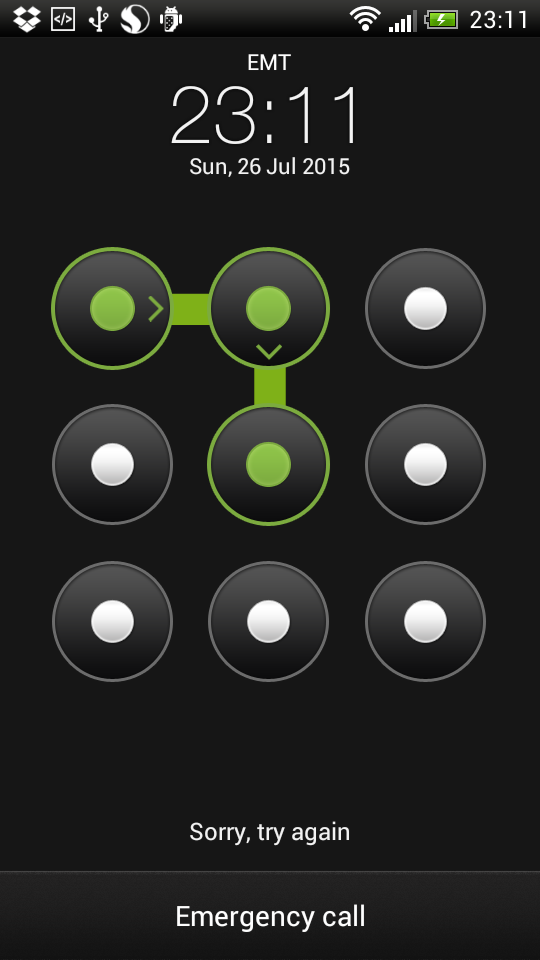
\includegraphics[width=0.35\textwidth]{images/lockpattern.png} \caption{Android lockpattern} \label{fig:android lockpattern} 
\end{center}
\end{wrapfigure}
As mentioned in the previous section a pattern is used to protect the credentials. Android users might already be familiar with the lockpattern even when they have not heard the term itself. It is used for locking the device from unwanted access to it, shown in the Figure 4.1. It is a 3x3 matrix consisting of circles/dots. To draw a pattern a user must press on a circle and drag through others to make a pattern and release to verify it. Even though the user only sees a picture of the pattern it is actually a string of numbers representing the dots where the user changed direction. For example a string "1-7-8" would be a pattern "L". 
Android lockpattern is known to users and is very easy to understand. Typing is taken out of the authentication process, which reduces the amount of errors made, and therefore used in this solution.

\section{Supporting Multiple Users}
The key factor what makes it different from previous solutions is the support for multiple users and multiple accounts per user. Mobile devices are commonly personal, but tablets in the other hand could be used in a household by the whole family. Needless to say that having to authenticate numerous times during a day might be a pain. 

\section{Data storage}
Every android comes with built in database system - SQLite \cite{sqlite}. It is easy to use, yet powerful to handle large amounts of data. Though no device will ever have the amount of users to even slightly test the database system, the benefit of using it is the simplicity and scalability allowing future changes in the database without losing any data already stored.

Since the library itself does not directly save data or query for it from the database, an Android component Content Provider \cite{contentprovider} is used. It manages access to the data, encapsulates it and provides mechanisms for defining data security. Content Providers can be used in two ways: provide access to it for all applications or just the one with permissions. In this case only the application intended to use it is given permissions declining any intruders from sniffing around.

\section{Structure of the library}
This section will go more specific into the structure, classes and flow of the library to give insight of how it works.

As mentioned numerous times previously, this solution is a library for Android applications. To be effective in the world of coding, reusing code made by self or others is essential. The same rule is implied here by using a library that withdraws the lockpattern function from Android source code. That is to say amongst other libraries used to create the final product of an application, these two libraries would be used in an application component tree as shown in the Figure 4.2.

\begin{figure}[h]
\begin{center}

\includegraphics[scale=0.9]{images/componentdiagram.png}
\caption{Example of application component diagram} \label{fig:component diagram} 
\end{center}
\end{figure}

The code within the library is somewhat sectioned: interface to the library, activities/visual presentation, content provider and database management. The most substantiate part of the code is database management with the highest complexity giving  the library flexibility. The database currently is located internally in the device, but the code is designed to allow moving it to another path on the device or entirely off to a cloud. All the data columns are defined in a "database contract" for easy access and modification, the database will automatically update itself if the underlying data model is changed and using singleton pattern only one instance of the database can run at any given time to prevent data corruption. The database management classe including the other classe can be seen in the class diagram in the Figure 4.3.

\begin{figure}[h]
\begin{center}
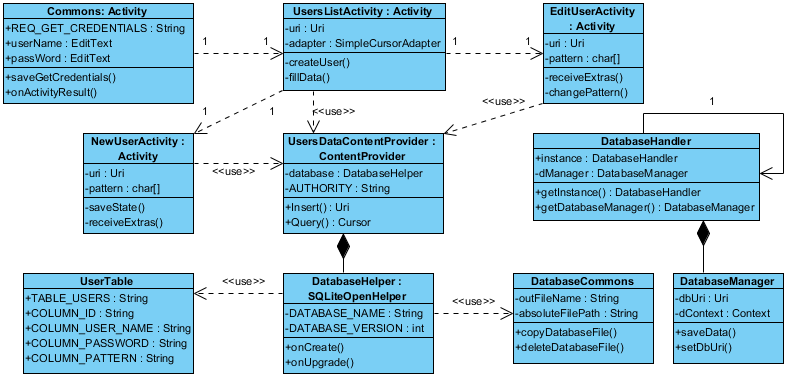
\includegraphics[scale=0.7]{images/classdiagram.png}
\caption{Class diagram of the library} \label{fig:class diagram} 
\end{center}
\end{figure}

The code within the library can also be divided into sections: interface to the library, activities/visual presentation, content provider and database management. It may seem much for so trivial task, every little component serves its purpose to 

Though applications and libraries are developed for present requirements, the future can not be foreseen and should always be somewhat considered. To make this library flexible to unseen changes design patterns are used. 

\section{Flow of the library}
To better understand what the library does, it is good to know the flow of it. For better visualisation a few diagrams are used.

Often less is more, this is the design ideal behind the library. A user has two main actions that he will take to authenticate: register an a account and start authenticating with it. In other words, one action is to get the credentials of the account into the phones memory and the other to access them.
 
When a user is logging into an application, using this library, he is asked whether he would like to save the credentials. If so he is taken to an activity to verify the password once more. When the password is verified, a new activity is presented to create a pattern for future authentication, and finally the credentials with the newly created pattern are stored to the database. This procedure is also illustrated on Figure 4.4 as a sequence diagram.

\begin{figure}[h]
\begin{center}
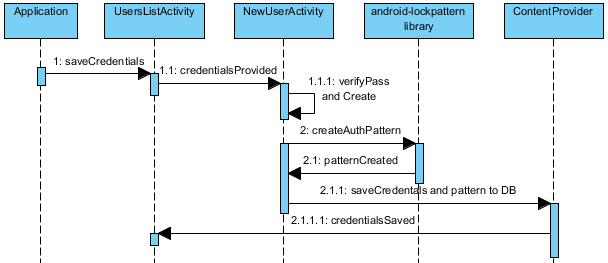
\includegraphics[scale=0.9]{images/sequencediagramnew.png}
\caption{Sequence diagram of registrating new account} \label{fig:sequence diagram} 
\end{center}
\end{figure}

With one or more credentials stored in the database the user can authenticate using them. Either finishing the registration sequence or accessing the UsersListAcivity from the the application, the user has a list of stored credentials presented to him. Clicking on a chosen account the library will get the information from the database and ask the user to verify the account by inputting the pattern. On a successful verification the credentials are passed to the application. Illustrative sequence diagram is shown on the Figure 4.5.

\begin{figure}[h!]
\begin{center}
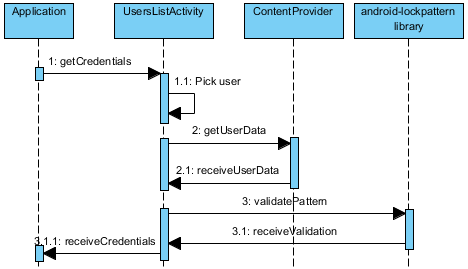
\includegraphics[scale=0.9]{images/sequencediagramauth.png}
\caption{Sequence diagram of authentication} \label{fig:sequence diagram} 
\end{center}
\end{figure}

\newpage
The previous descriptions and sequence diagrams of the registration and authentication process give the idea of a successful interpretation of the library. Though the user is given choices to back out of the process or the process could be failed. A flow chart covering these possibilities is seen in the Figure 4.6.

\begin{figure}[h!]
\begin{center}
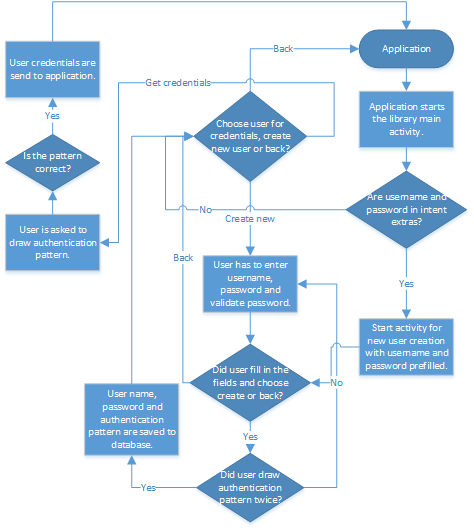
\includegraphics[scale=1]{images/flowchart.png}
\caption{Flow chart of registration and authentication process} 
\label{fig:flow chart} 
\end{center}
\end{figure}

\section{Importing the library into a project}
This section is describing how to include this library in a project in terms of getting the library in a workspace and a code sample.



\section{Summary}
Summarize the chapter with at least two paragraphs.



% ---------------------------------------------------------------------------
%: ----------------------- end of thesis sub-document ------------------------
% ---------------------------------------------------------------------------

		% how the solution solved the problem - your solution
% this file is called up by thesis.tex
% content in this file will be fed into the main document

%: ----------------------- name of chapter  -------------------------
\chapter{Case Studies} % top level followed by section, subsection


Typing on a smartphone is made easier to the user by including auto-correct, but the same tool can not be used for authentication process. Therefore users are left with the task to hit every key accurately or repeat the task until they get it right. 

In this chapter we present the results from a survey made to determine, whether the proposed authentication method increases the user experience.


%: ----------------------- paths to graphics ------------------------

% change according to folder and file names
\ifpdf
    \graphicspath{{X/figures/PNG/}{X/figures/PDF/}{X/figures/}}
\else
    \graphicspath{{X/figures/EPS/}{X/figures/}}
\fi

%: ----------------------- contents from here ------------------------

\section{Validation}
In order to validate the hypothesis, the proposed solution is compared to the conventional ''input credentials'' method in terms of simplicity and user experience. A use case based on social media sign-in was developed. The application is primitive to only test the authentication process. 

In the validation, a tablet LG G Pad 8.3 \footnote[16]{http://www.gsmarena.com/lg\_g\_pad\_8\_3-5673.php} was used. It has a 8.3 inch screen with the resolution of 1200x1920 pixels and is running Android 4.4.2, otherwise called as KitKat \footnote[17]{https://www.android.com/versions/kit-kat-4-4/}.

\subsection{Experimental Setup}
	
In the first application, only the conventional method is used as shown in Figure 5.1. The second application uses the proposed solution, which is divided into two parts: registering an account and authenticating with the stored account. Screenshots of the credentials saving process are seen in Figure 5.2. Once the library is integrated within the app, a button \textit{Save/Get Credentials} appears (1). With the username and password filled in, pressing the mentioned button, the user is requested to validate his password by typing it for the second time (2). Pressing the button \textit{Create}, the user can introduce a pattern (3), after drawing it twice, the process of credentials registration is complete and the user is taken to a list of accounts already stored (4). Screenshots of the authentication sequence are seen in Figure 5.3. The second step of authentication will either start from where registration ended or from a newly opened applications empty main page (1). Pressing the \textit{Save/Get Credentials} button, a list of stored accounts is presented to the user (2). Selecting an account in the list, the user is prompted to draw a pattern (3) and on a successful authentication the user is taken back to the main page with the username and password filled in (4).

To compare these two methods, a questionnaire was composed |Appendix A|. It consists of 10 questions, first 2 are general questions about participants satisfactory to authentication process today. The next two sections, questions 3-6 and 7-10, are more specific to the authentication methods implied to applications used in this case study. 

\subsection{Methodology}
There were 20 participants between the ages of 20 and 30, all day-to-day smartphone users. None of them have expertise in computer science, hence they are only end users. They were asked to first answer the first two questions, then they would perform authentication on the application with the conventional method and respond to question 3-6. Then they would register an account and authenticate themselves with the second application, also change the stored password or pattern and answer the last four questions. 

\begin{figure}[H]
\centering
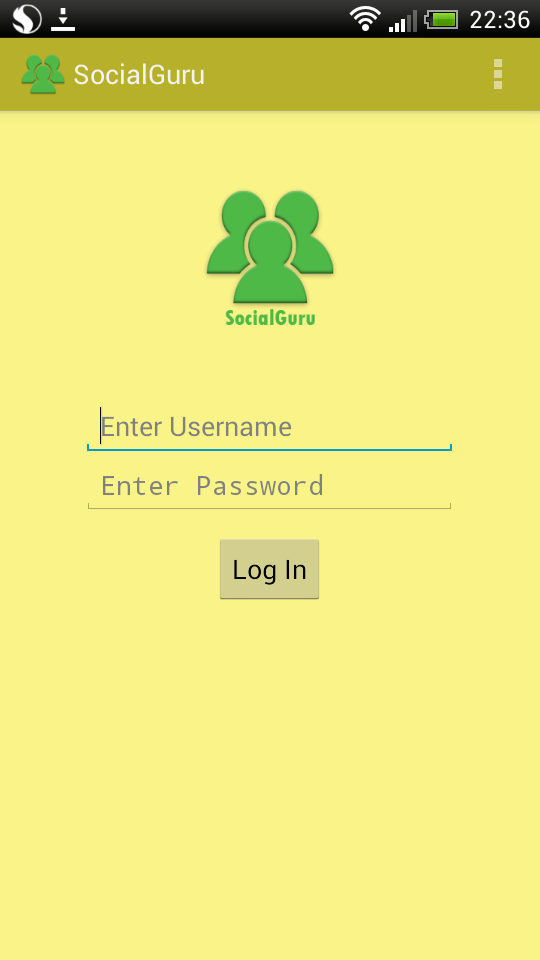
\includegraphics[scale=0.3]{images/nolibrary.png}
\caption{Application with only conventional method.}
\label{fig:nolibrary}
\end{figure}

\begin{figure}[H]
\begin{center}
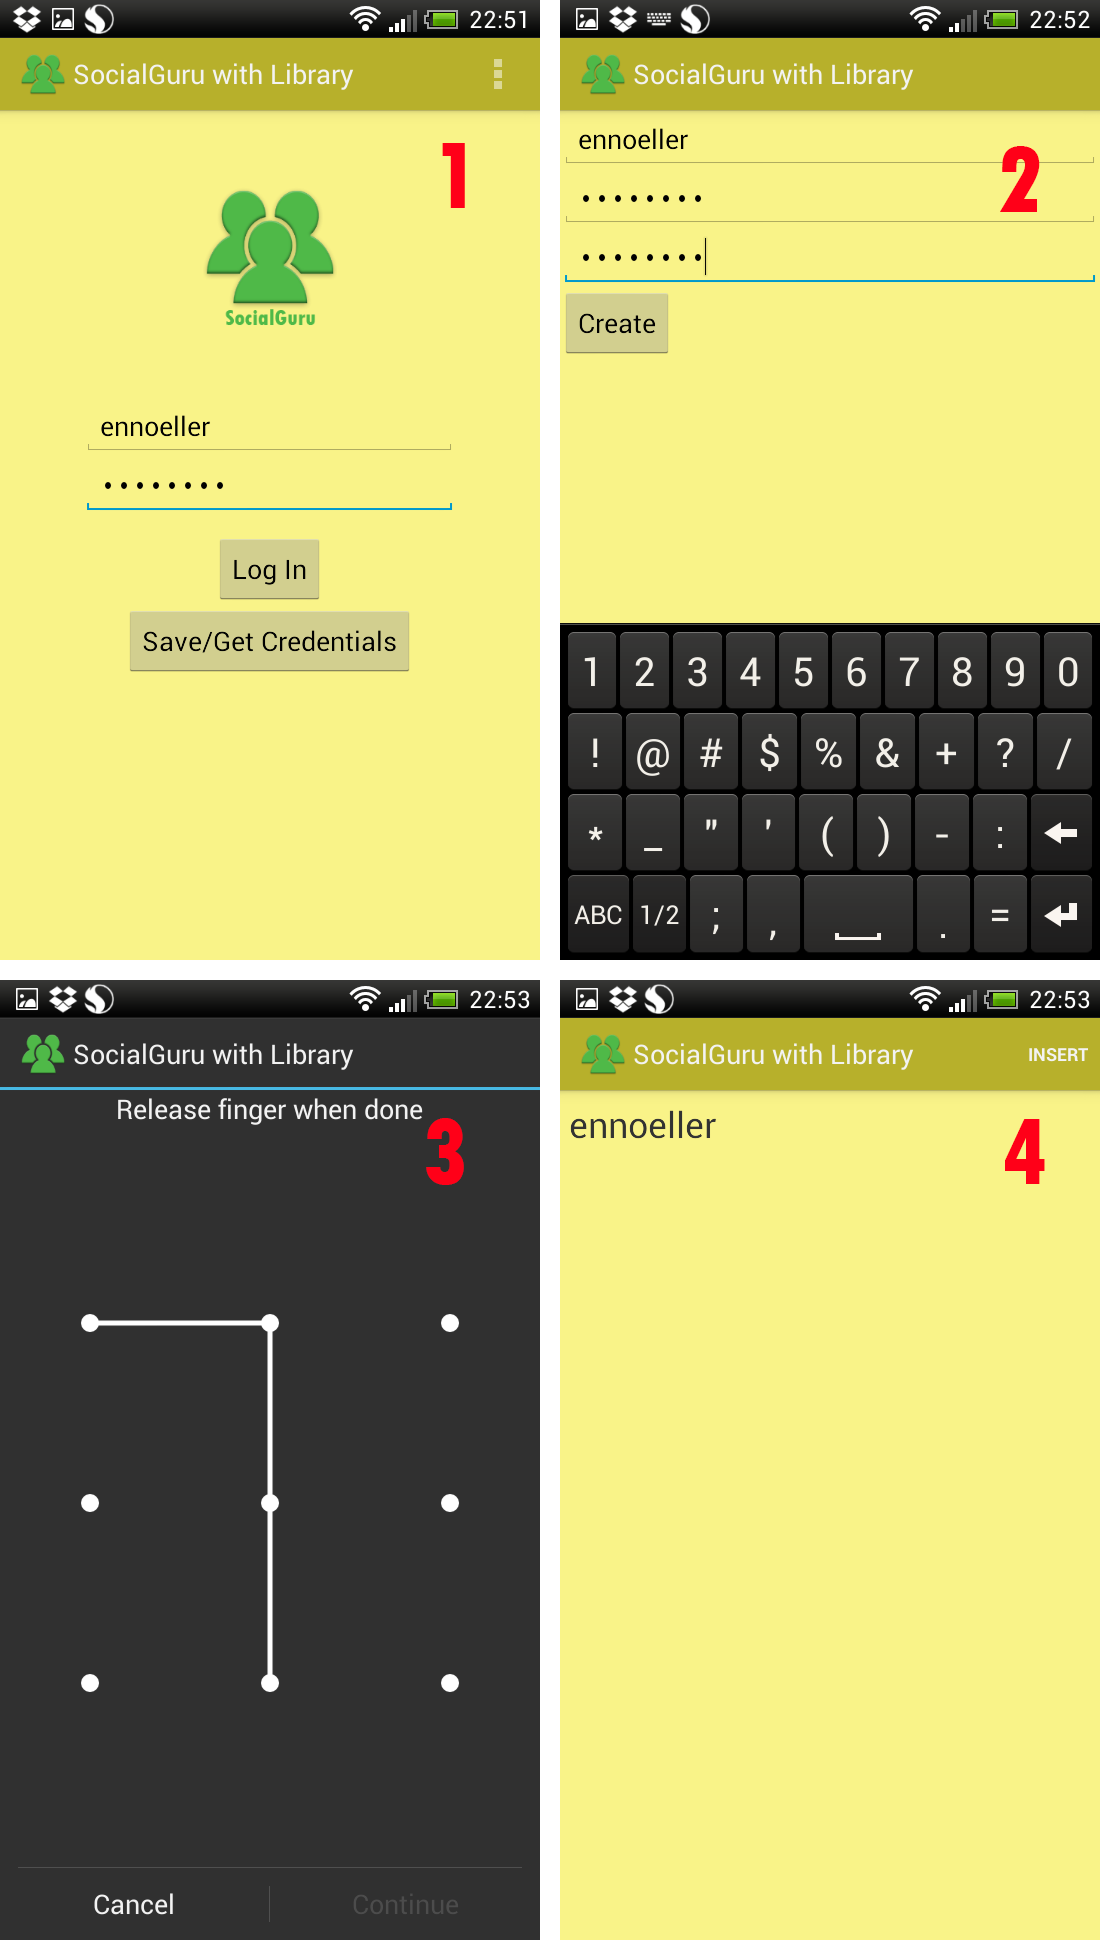
\includegraphics[scale=0.3]{images/reg.png}
\caption{Credentials saving process with the library.}
\label{fig:credentials saving}
\end{center}
\end{figure}

\begin{figure}[H]
\begin{center}
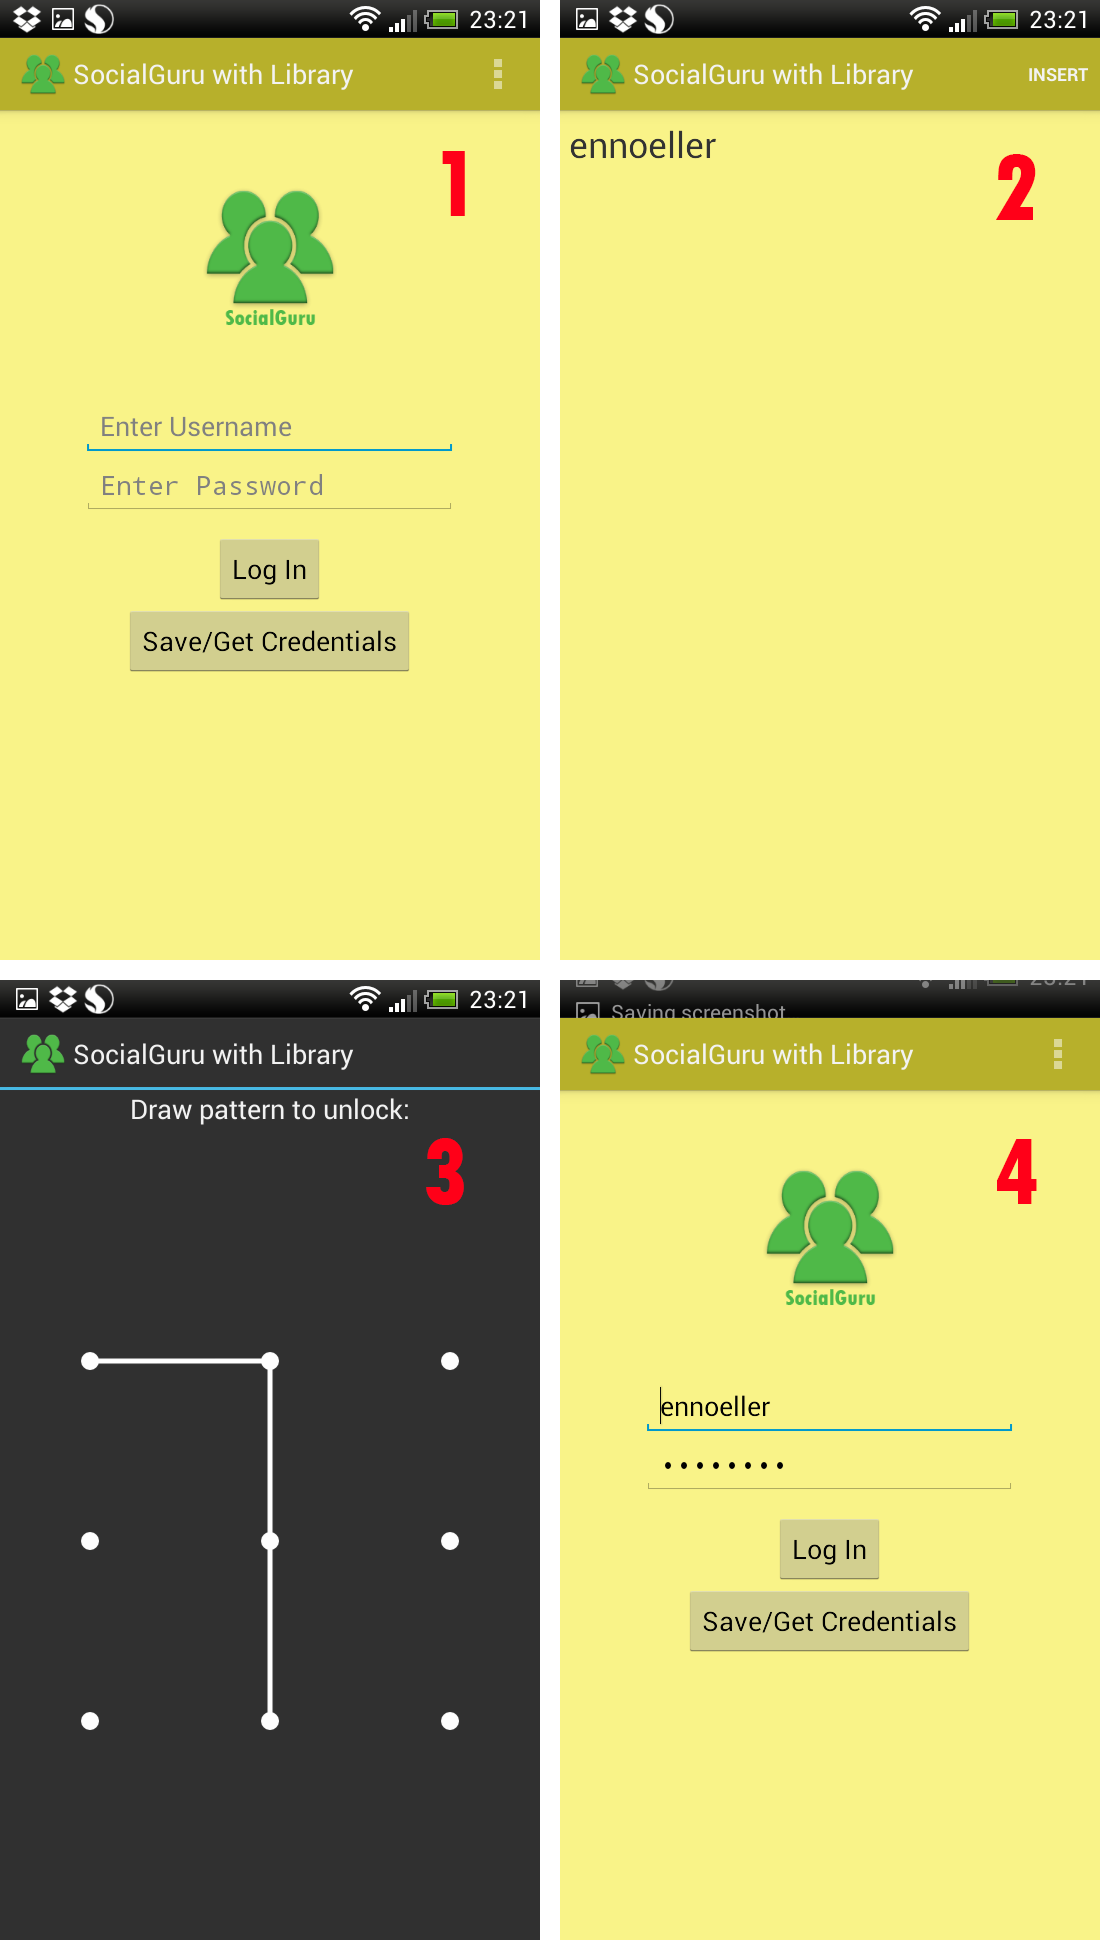
\includegraphics[scale=0.3]{images/auth.png}
\caption{Athentication process with the library.}
\label{fig:authentication}
\end{center}
\end{figure}

\section{Results}

First two questions were about participants opinions about authentication methods used in applications. 65\% of them, shown in Figure 5.4, find that applications do use suitable login methods. 5 out of 7 participants, who find applications not to use suitable methods, brought out that the process should include less typing. 

\begin{figure}[H]
\centering
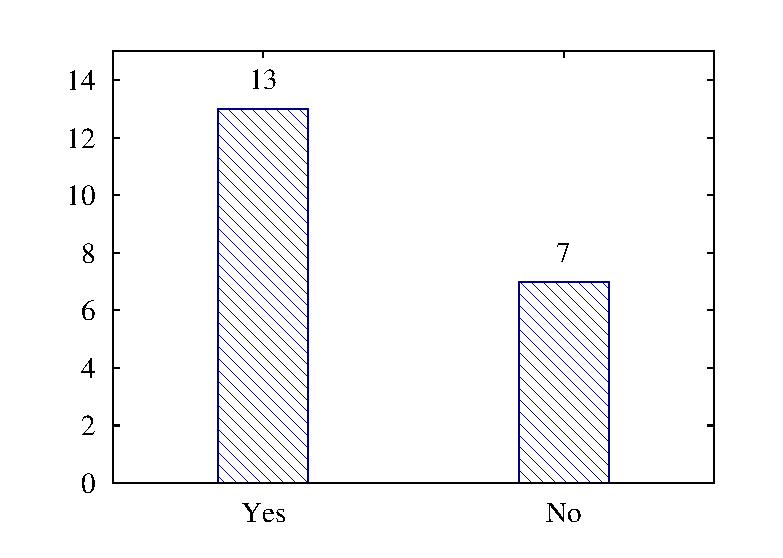
\includegraphics[scale=.7]{files/question1/question1.eps}
\caption{Participants satisfaction with the login methods used in apps.}
\label{fig:digraph}
\end{figure}

\subsection{Participants Opinion on Conventional Login}
Most of the participants found the authentication method to be normal (45\%) or even hard (34\%) for them as seen on the Figure 5.5, implying to the size of the keyboard on the device. Similar results applied to the question of, whether they were annoyed by the process, shown at Figure 5.6. Given the answers values of 1 to 3, 1 being ''Easy/Low'', the average to both of these questing would be 2.15. 

As seen from the Figures 5.7 and 5.8, the conventional login method would push users away from the application or make them change their passwords to something easier to type. 35\% of the participants would definitely use the application less and 30\% are considering it, making the application less appealing to 65\% of users because of the authentication process. This method is also pushing 70\% of the  users to change their passwords, making them more vulnerable to intruders.  

This shows how damaging the conventional method could be for the user base and reputation of the application. Also users are put to danger by allowing themselves to use weaker passwords.

\begin{figure}[H]
\centering
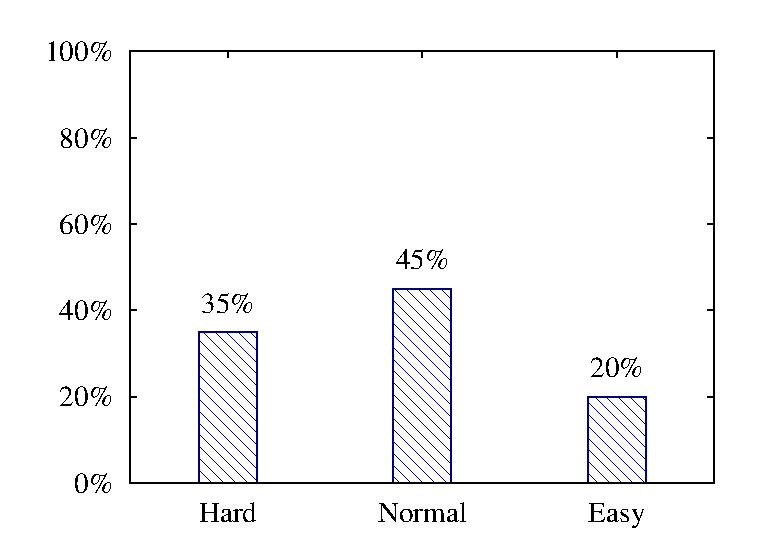
\includegraphics[scale=.7]{files/question3/question3.eps}
\caption{Complexity in the authentication process with conventional method.}
\label{fig:digraph}
\end{figure}

\begin{figure}[H]
\centering
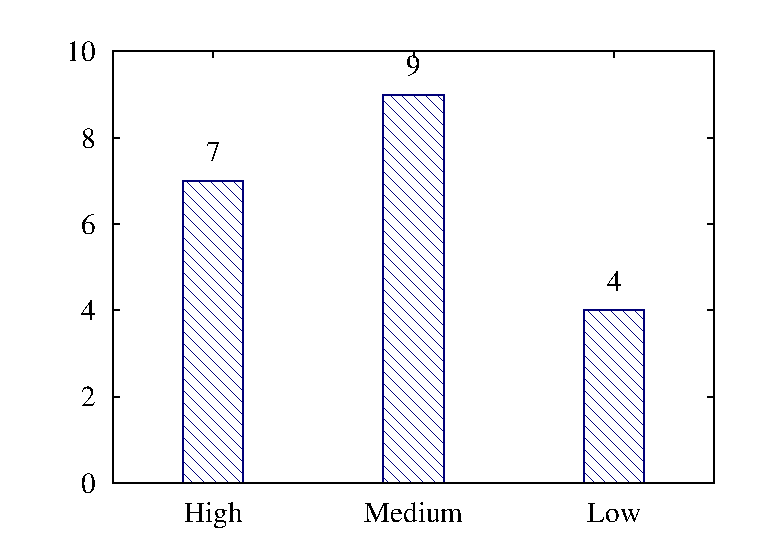
\includegraphics[scale=.7]{files/question4/question4.eps}
\caption{Level of annoyance caused by conventional method.}
\label{fig:digraph}
\end{figure}

\begin{figure}[H]
\centering
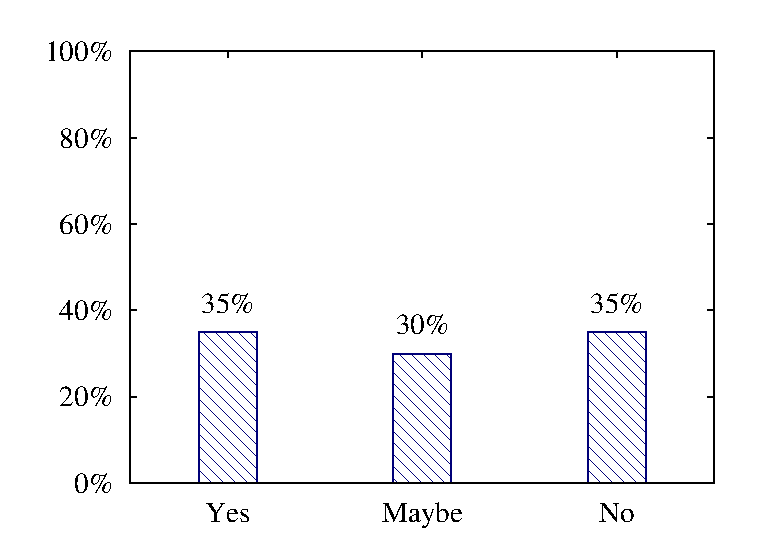
\includegraphics[scale=.7]{files/question5/question5.eps}
\caption{Participants being pushed away by the inconvenience.}
\label{fig:digraph}
\end{figure}

\begin{figure}[H]
\centering
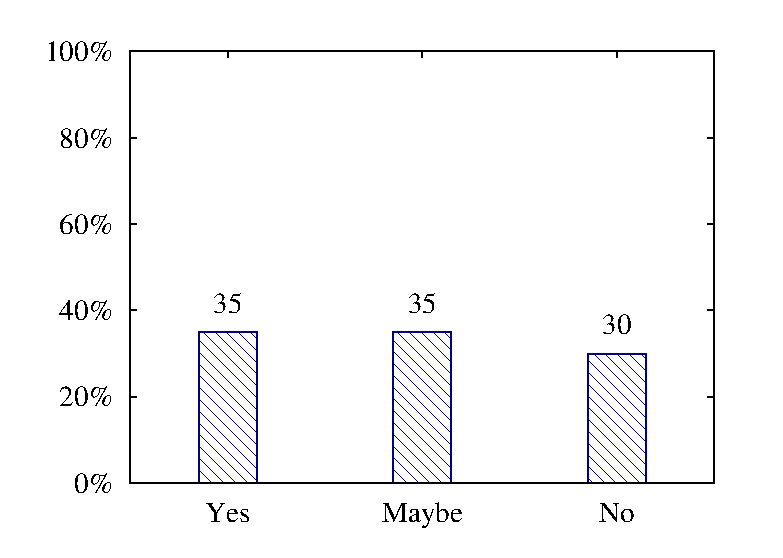
\includegraphics[scale=.7]{files/question6/question6.eps}
\caption{Discomfort making users change their passwords. }
\label{fig:digraph}
\end{figure}

\subsection{Participants Opinion on the Proposed Solution}

The participants were using this method for the first time and were asked questions about the simplicity of it, to see whether this solution could be justified. 

Compared to the conventional method, the proposed solution seems to be easier to use, see the Figure 5.9. Nobody thought it was hard. 75\% of the participants found the method easy and 25\% normal. Given the answers values of 1 to 3, 1 being ''Easy'', the average would be 1.25. This is also reflected on usage of the application, where nobody answered they would definitely use the application less, shown on Figure 5.10, because of the provided method. Only 15\% of participants would consider using it less. 

The given method was composed of two steps. Before authenticating themselves, they had to register their credentials with the application. 75\% of the participants found the process easy and nobody felt confused, as seen on Figure 5.11. When asked to change the password or pattern saved in the application, some participants felt confused in the process - 25\%, but 55\% found it intuitive, as seen in Figure 5.12.

\begin{figure}[H]
\centering
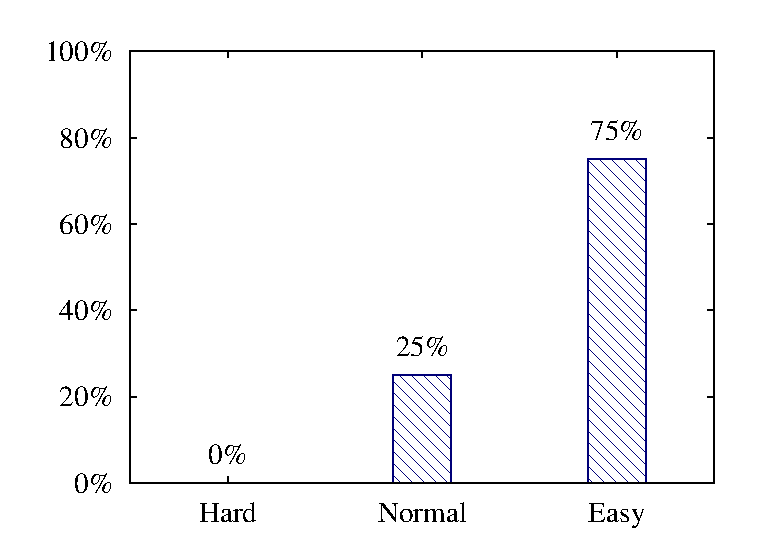
\includegraphics[scale=.7]{files/question7/question7.eps}
\caption{Complexity in the authentication process with pattern based method.}
\label{fig:digraph}
\end{figure}

\begin{figure}[H]
\centering
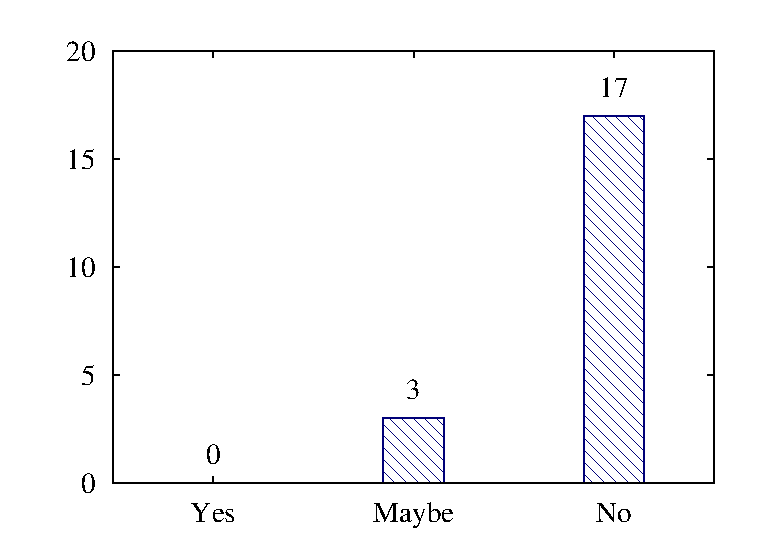
\includegraphics[scale=.7]{files/question8/question8.eps}
\caption{Participants being pushed away by the discomfort.}
\label{fig:digraph}
\end{figure}

\begin{figure}[H]
\centering
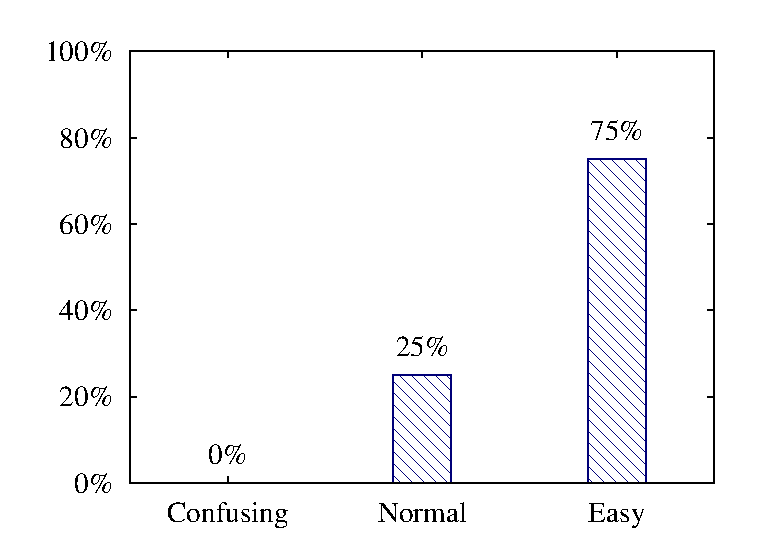
\includegraphics[scale=.7]{files/question9/question9.eps}
\caption{Simplicity of the credentials saving process.}
\label{fig:digraph}
\end{figure}

\begin{figure}[H]
\centering
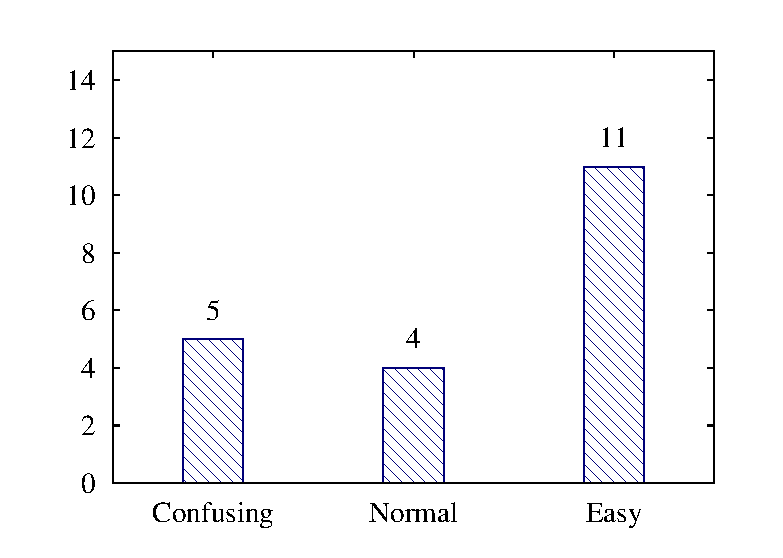
\includegraphics[scale=.7]{files/question10/question10.eps}
\caption{Simplicity of the password or pattern changing process.}
\label{fig:digraph}
\end{figure}

\section{Summary}
In this chapter the usability of the proposed mechanism is validated.  With the conventional model, 35\% of the participants found it hard and annoying. 65\% of participants felt the process to be repulsive and 70\% sensed the need to change their passwords to something easier to type, therefore less secure. Opposed to the conventional method, the proposed solution was easier to the user, as 75\% of the participants found it easy to use and therefore they were not losing interest in the application, as only 15\% found it slightly repulsive. To store credentials, users have register their credentials and sometimes change their passwords. Although these are additional steps in the process, most participants find them easy to complete.



% ---------------------------------------------------------------------------
%: ----------------------- end of thesis sub-document ------------------------
% ---------------------------------------------------------------------------

			% functional scenario
% this file is called up by thesis.tex
% content in this file will be fed into the main document

%: ----------------------- name of chapter  -------------------------
\chapter{Conclusions and Future Directions} % top level followed by section, subsection
Summarize your work and results.



%: ----------------------- paths to graphics ------------------------

% change according to folder and file names
\ifpdf
    \graphicspath{{X/figures/PNG/}{X/figures/PDF/}{X/figures/}}
\else
    \graphicspath{{X/figures/EPS/}{X/figures/}}
\fi

%: ----------------------- contents from here ------------------------







% ---------------------------------------------------------------------------
%: ----------------------- end of thesis sub-document ------------------------
% ---------------------------------------------------------------------------

			% final conclusions
\include{6/relatedwork}	                % related work
\include{6/futureresearch}		% future research directions
\include{7/eestiabstract}               % discussion of results



% --------------------------------------------------------------
%:                  BACK MATTER: appendices, refs,..
% --------------------------------------------------------------

% the back matter: appendix and references close the thesis


%: ----------------------- bibliography ------------------------

% The section below defines how references are listed and formatted
% The default below is 2 columns, small font, complete author names.
% Entries are also linked back to the page number in the text and to external URL if provided in the BibTex file.

% PhDbiblio-url2 = names small caps, title bold & hyperlinked, link to page 
%\begin{multicols}{2} % \begin{multicols}{ # columns}[ header text][ space]
\begin{tiny} % tiny(5) < scriptsize(7) < footnotesize(8) < small (9)

%\bibliographystyle{Latex/Classes/PhDbiblio-url2} % Title is link if provided
%\renewcommand{\bibname}{References} % changes the header; default: Bibliography

%\bibliography{9_backmatter/references} % adjust this to fit your BibTex file


\bibliographystyle{elsarticle-num}	% references style
\bibliography{thesis}			% references bibtex file  - utilize JabRef

\end{tiny}
%\end{multicols}

% --------------------------------------------------------------
% Various bibliography styles exit. Replace above style as desired.

% in-text refs: (1) (1; 2)
% ref list: alphabetical; author(s) in small caps; initials last name; page(s)
%\bibliographystyle{Latex/Classes/PhDbiblio-case} % title forced lower case
%\bibliographystyle{Latex/Classes/PhDbiblio-bold} % title as in bibtex but bold
%\bibliographystyle{Latex/Classes/PhDbiblio-url} % bold + www link if provided

%\bibliographystyle{Latex/Classes/jmb} % calls style file jmb.bst
% in-text refs: author (year) without brackets
% ref list: alphabetical; author(s) in normal font; last name, initials; page(s)

%\bibliographystyle{plainnat} % calls style file plainnat.bst
% in-text refs: author (year) without brackets
% (this works with package natbib)


% --------------------------------------------------------------

% according to Dresden med fac summary has to be at the end
%\noindent\textbf{\large Simplifying Mobile Social Media Authentication On Android}
\vspace*{2ex}
{\flushleft{\textbf{Abstract:}}}

\noindent Nowadays, smartphones are very common and people all around the world are using them in their everyday life. Even though mobile phones were originally invented as calling devices, smartphones allow the user to communicate in different ways including social media, instant messaging, recording and watching videos, etc. Recent statistics as of January 2014 claim, that 74\% of online adults use social media. In case they own a smartphone, they probably use social media on it as well, but with restrictions that come with the size of the device, affecting how we view content and also type. Typing on smartphones can be frustrating, but more so when the keyboard size prevents us from succeeding with authentication and we have to type the same text numerous times, which can lead to shorter passwords decreasing the security of the accounts. This paper proposes a solution to such occurrences by using pattern recognition rather than typing. Patterns allow the screen to be used more efficiently, giving the user more room for accuracy errors. Survey results indicate that approaching authentication in this way is feasible.

\vspace*{2ex}

{\flushleft{\textbf{Keywords:} Mobile, Android, Authentication, Pattern}}

\vspace*{3ex}

\noindent\textbf{\large Mobiilse Sotsiaalmeedia Autentimise Lihtsustamine Androidil}
\vspace*{2ex}
{\flushleft{\textbf{L\"{u}hikokkuv\~{o}te:}}}

\noindent T\"{a}nap\"{a}eval on nutitelefonid v\"{a}ga levinud ja k\~{o}ikjal maailmas inimesed kasutavad neid oma igap\"{a}eva elus. Kuigi mobiiltelefonid loodi algselt helistamiseks, nutitelefonid v\~{o}imaldavad kasutajal suhelda erinevatel viisidel, nende seas sotsiaalmeedia, kiirs\~{o}numid, lindistada ja vaadata videoid jne. Hiljutised uuringud jaanuarist 2014 v\"{a}idavad, et 74\% internetti kasutavatest t\"{a}isealistest tarvitavad ka sotsiaalset meediat. Juhul, kui need isikud omavad nutitelefoni, on t\~{o}en\"{a}osus, et nad kasutavad sotsiaalmeediaid ka oma nutiseadmel, kuid piirangutega, mis tulenevad seadme suurusest. Suurus m\~{o}jutab, kuidas me infot vaatame ja teksti sisestame. Tr\"{u}kkimine nutitelefonil v\~{o}ib osutuda masendavaks, seda enam, kui klaviatuuri suurus takistab meil autentimise edu ja me peame sama teksti sisestama mitmeid kordi. Sellised olukorrad v\~{o}ivad viia l\"{u}hemate paroolide kasutamiseni, mis omakorda v\"{a}hendab meie kontode turvalisust. Antud t\"{o}\"{o} pakub v\"{a}lja lahenduse sellistele olukordadele kasutades tr\"{u}kkimise asemel mustreid. Mustrid v\~{o}imaldavad efektiivsemat ekraani kasutust, mis annavad kasutajale rohkem ruumi t\"{a}psuse vigade v\"{a}ltimiseks. Uuringu tulemused n\"{a}itavad, et selline l\"{a}henemine autentimisele on v\~{o}imalik.

\vspace*{2ex}

{\flushleft{\textbf{V\~{o}tmes\~{o}nad:} Mobiilne, Android, Autentimine, Muster}}

%: Declaration of originality
%\include{9_backmatter/declaration}



\end{document}
